\bchapter{Object Detection}
Al fine di comprendere a pieno e dimostrare l’utilizzo di un framework per l’implementazione di modelli di machine learning su dispositivi mobili, abbiamo
realizzato un’applicazione che ne fa uso: \textbf{ObjectDetection}.

Abbiamo scelto di utilizzare \textbf{TensorFlow} per la sua efficienza e per la maggiore disponibilità di esempi e di modelli pre-allenati di cui dispone.

L’applicazione è in grado, tramite la fotocamera frontale, di individuare e classificare gli oggetti che vede. Oltre alla classificazione, ObjectDetection
fornisce le Bounding Boxes (rettangoli) che delimitano gli oggetti e i punteggi di confidenza in merito alla sicurezza del modello sulle classificazioni fatte.
\begin{figure}
    \centering
    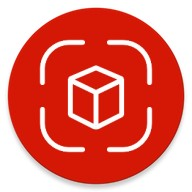
\includegraphics[width=0.3\textwidth]{Immagini/App/icona_app.jpg}
    \caption{Logo dell’app}
\end{figure}

\newpage
\section{Struttura dell'applicazione}
ObjectDetection è formata da 3 componenti principali: il primo è costituito dalle activity che si occupano di \textbf{Login} (accesso, registrazione e recupero
password), il secondo consiste in tutte le activity e le classi utilizzate per gestire la \textbf{home} dell’app e il terzo componente riguarda la gestione della
\textbf{fotocamera} e l’effettiva implementazione del modello.
L’applicazione lega e sfrutta a pieno queste 3 componenti per garantire un utilizzo scorrevole e una larga gamma di funzionalità che arricchiscono
l’esperienza dell’utente.

\subsection{Home}
La home di ObjectDetection consiste in due schermate principali: l’effettiva home e una schermata informativa (\textbf{Info}).
Una volta nella home, l’utente ha due possibilità: avviare la fotocamera e iniziare a identificare e classificare oggetti premendo sul pulsante
“\textit{Get started!}” oppure cliccare su Home aprendo un menu a tendina (\textbf{Spinner}) che fornisce le seguenti opzioni (visibili in figura \ref{fig:home}):
\begin{itemize}
    \item Info: avvia l’interfaccia informativa che fornisce dettagli sul funzionamento del modello;
    \item Change theme: cambia il tema grafico dell’applicazione; 
    \item Logout: esegui il logout dell'utente e ritorna alla schermata di Autenticazione.
\end{itemize}

\subsection{Info}
ObjectDetection fornisce una schermata informativa (Info) allo scopo di dettagliare all’utente il funzionamento dell’applicazione e del modello TensorFlow
Lite usato nell'app.
Anche in questo caso, è possibile cliccare lo spinner in alto a destra e accedere a tutte le funzionalità prima citate. Naturalmente, cliccare l’opzione
Info non comporterà alcuna azione e cliccando l’opzione Home (oppure cliccando il pulsante del proprio telefono per tornare indietro) si ritornerà alla schermata di home.

Le informazioni contenute in questa schermata (figura \ref{fig:info}) sono più di quanto essa riesca a contenere, per questo la schermata ne visualizza solo una parte e l’utente
ha la possibilità di scrollare in basso per visualizzare tutto il contenuto di questa interfaccia.

\subsection{Cambio tema}
ObjectDetection fornisce, inoltre, la possibilità di cambiare il tema cromatico dell’applicazione. Fino ad ora, le schermate presentate erano tutte nel
tema \textbf{LIGHT}, realizzato in modo da essere chiaro e leggero alla vista. L’app dispone anche del tema \textbf{DARK} che presenta colori più marcati e contrastanti tra
loro (figure \ref{fig:dark1} e \ref{fig:dark2}).
Il cambio del tema si applica anche a tutti i vari widget presenti nella UI per garantire un aspetto più coerente con il tema scelto.

\section{Orientamento}
In tutte le schermate dell’app, ObjectDetection supporta anche l’orientamento orizzontale completando piacevolmente l’esperienza dell’utente.
Nel cambio di configurazione, il design complessivo e le funzionalità dell’app rimangono immutate ma la disposizione e la struttura delle schermate varia
per adattarsi al nuovo orientamento del dispositivo (figure \ref{fig:orizzontale1} e \ref{fig:orizzontale2}).

\section{Get Started!}
A seguito di questa breve descrizione strutturale, è utile mostrare alcuni esempi di utilizzo di ObjectDetection in modo da comprendere a pieno come
funziona e quali servizi offre.
Dopo aver aperto l’app ed aver effettuato il login, cliccando il pulsante “Get started!” ObjectDetection accederà alla telecamera del dispositivo (previa autorizzazione da parte dell'utente) per iniziare 
identificare oggetti.
La fotocamera usata è quella frontale e l’applicazione riconosce e classifica tutta una serie di oggetti (per i quali il modello è stato addestrato) che gli si presentano davanti.
Durante l’utilizzo dell’applicazione, è possibile aprire un menu a tendina dal basso con le seguenti opzioni:
\begin{itemize}
    \item Valore di soglia: il minimo punteggio di confidenza di cui deve disporre un oggetto classificato per mostrare la sua identificazione su schermo;
    \item Max rettangoli: il numero massimo di oggetti (e quindi di bounding boxes) che vogliamo classificare per volta. È utile per evitare che
    l’applicazione riconosca eccessivi oggetti causando un’esperienza visiva meno gradevole;
    \item Delegato: il tipo di delegato usato nell’utilizzo del modello. Si può scegliere tra CPU, GPU e NNAPI.
\end{itemize}
Nell’esempio visibile in figura \ref{fig:funzionamento1}, l’applicazione riconosce correttamente il microonde, il telefono e la mano (classificata come persona) usando il delegato CPU.
Il numero di rettangoli massimi è 3 e il valore di soglia minimo è 0.5, infatti ciascun oggetto ha un punteggio di confidenza strettamente maggiore alla
soglia impostata.
In figura \ref{fig:funzionamento2} è possibile vedere un esempio con valore di soglia uguale ma numero massimo di rettangoli pari a 4.
Come ci si aspettava, l’app riconosce correttamente quattro oggetti.
È bene notare che, in quest’ultimo esempio, il microonde non è inquadrato totalmente, il telefono è capovolto e si vede anche l’avambraccio della persona.
Tutti questi cambiamenti incidono sul punteggio di confidenza attribuito dal modello: il microonde ha un valore minore, la persona maggiore,
mentre il telefono rimane più o meno allo stesso valore.

\begin{figure}[ht]
    \centering
    \begin{subfigure}[b]{0.3\textwidth}
      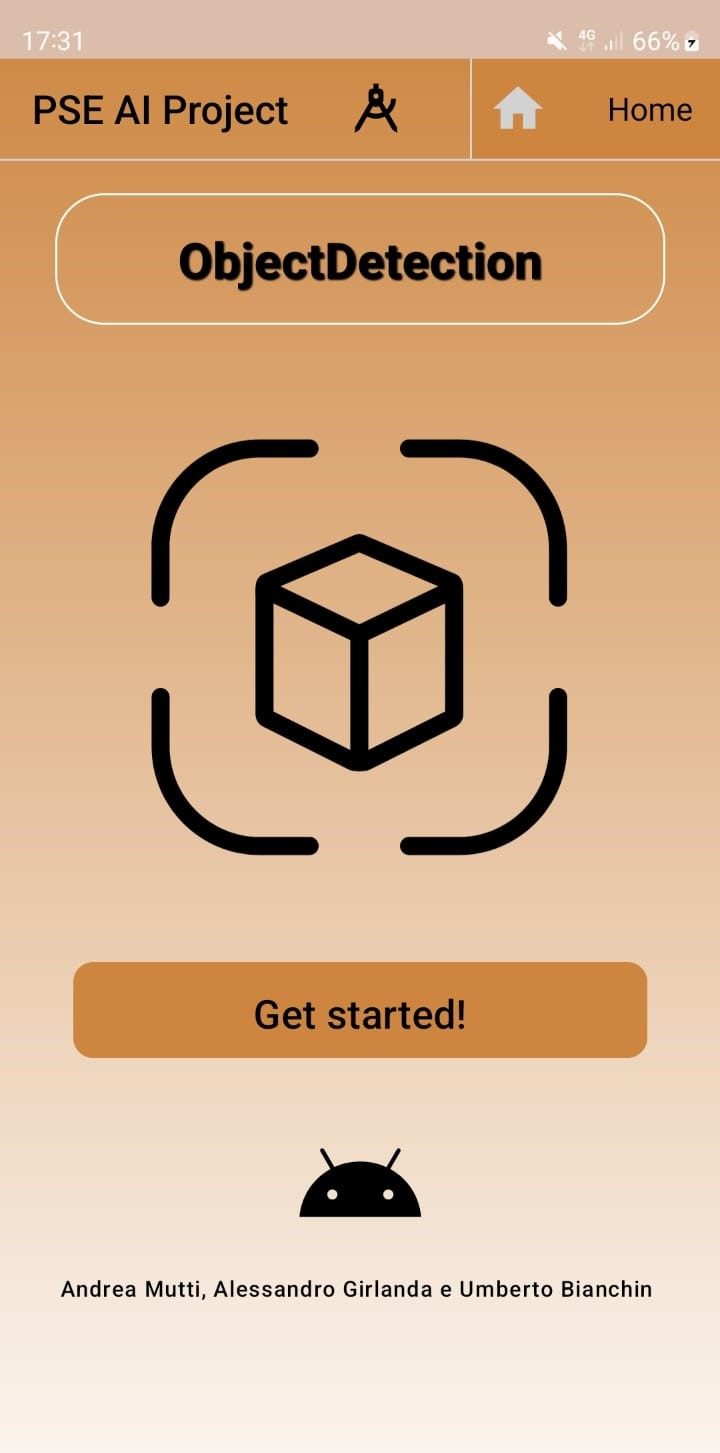
\includegraphics[width=\textwidth, height=0.45\textheight]{Immagini/App/home_chiaro.jpeg}
    \end{subfigure}
    \begin{subfigure}[b]{0.3\textwidth}
      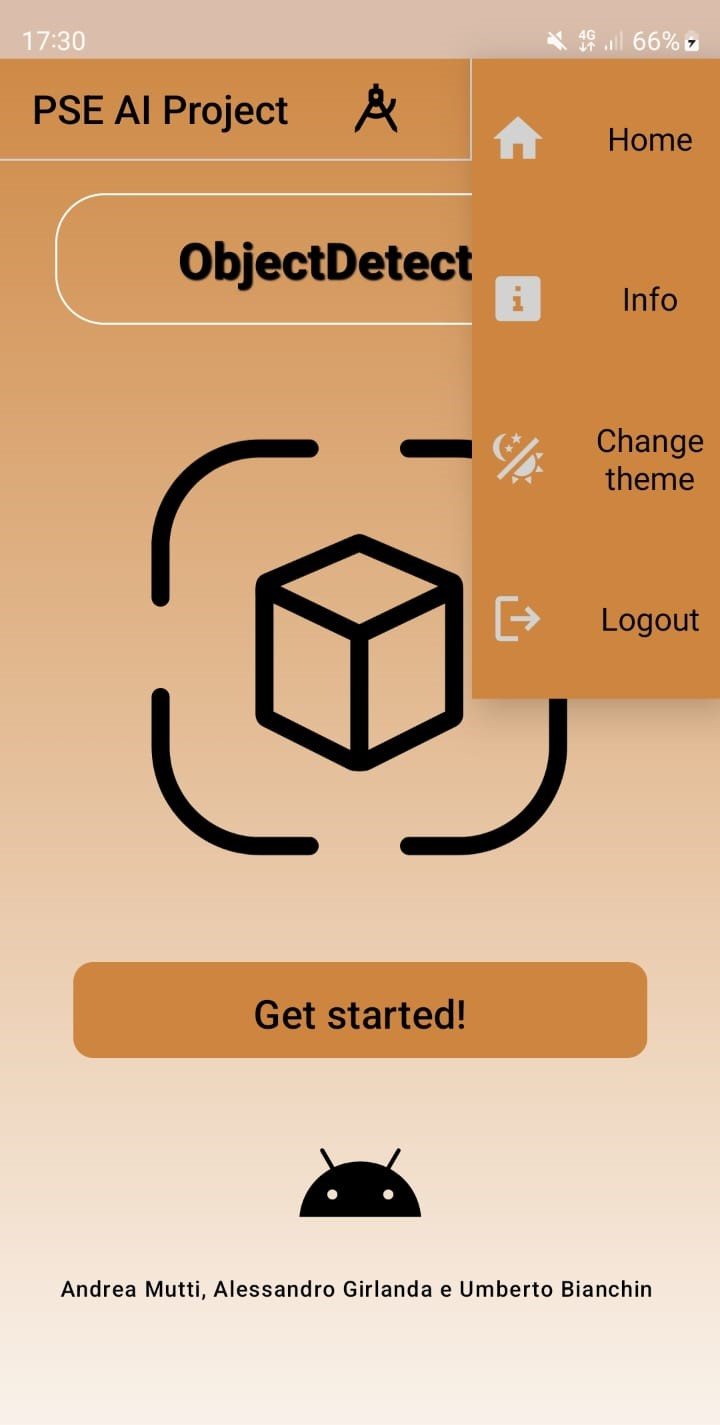
\includegraphics[width=\textwidth, height=0.45\textheight]{Immagini/App/home_spinner_chiaro.jpeg}
    \end{subfigure}
    \caption{Schermata home e apertura dello spinner.}
    \label{fig:home}
\end{figure}

\begin{figure}[ht]
    \centering
    \begin{subfigure}[b]{0.3\textwidth}
      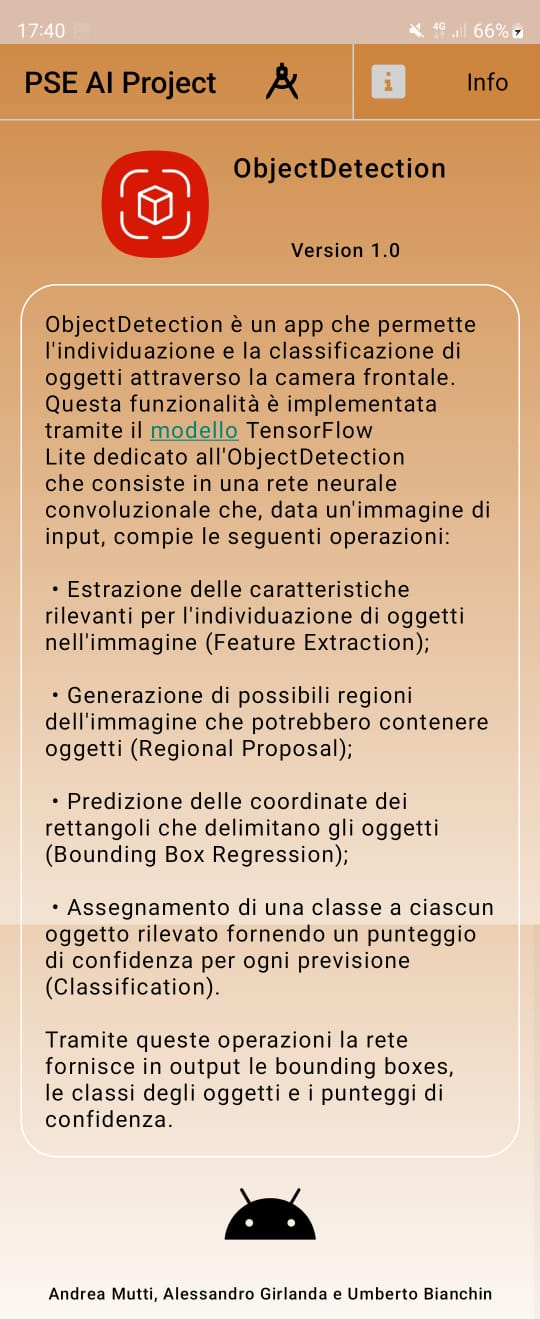
\includegraphics[width=\textwidth, height=0.45\textheight]{Immagini/App/info_chiaro.jpeg}
    \end{subfigure}
    \begin{subfigure}[b]{0.3\textwidth}
      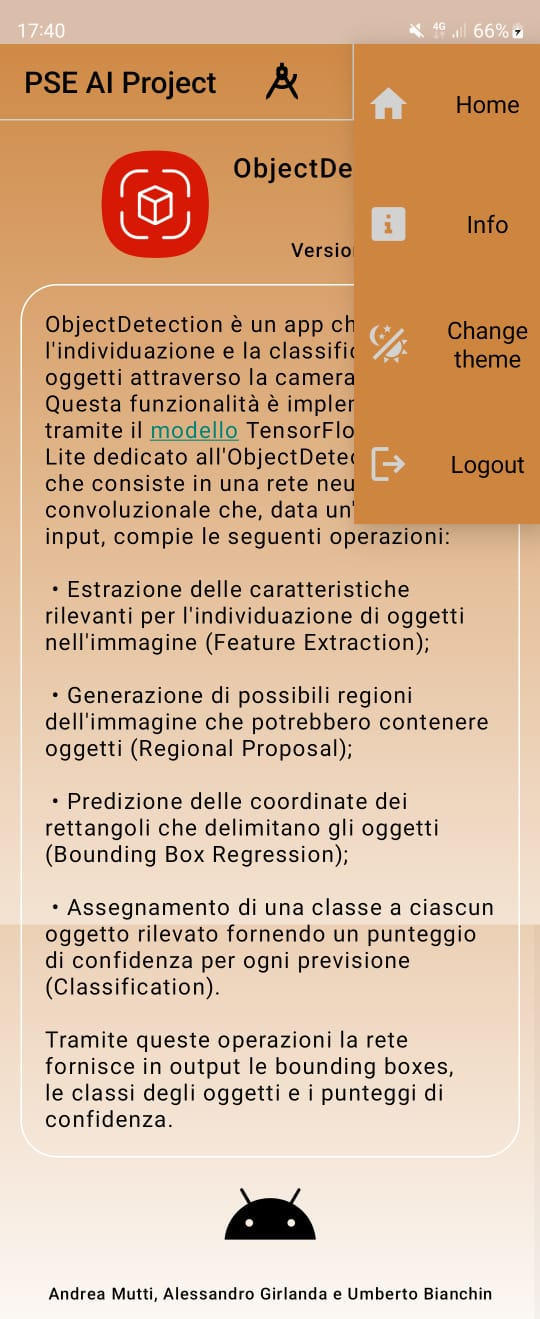
\includegraphics[width=\textwidth, height=0.45\textheight]{Immagini/App/info_spinner_chiaro.jpeg}
    \end{subfigure}
    \caption{Schermata info e apertura dello spinner.}
    \label{fig:info}
\end{figure}

\begin{figure}[ht]
    \centering
    \begin{subfigure}[b]{0.3\textwidth}
      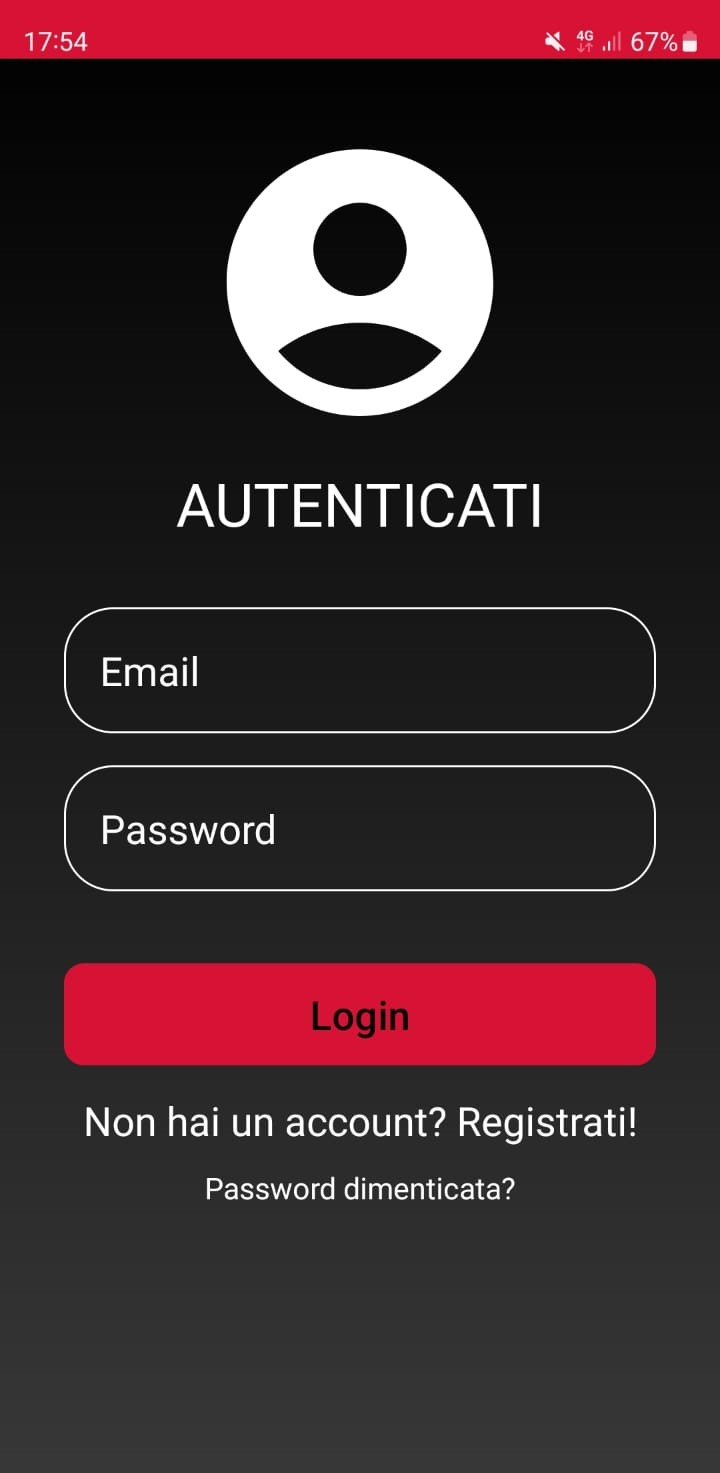
\includegraphics[width=\textwidth, height=0.45\textheight]{Immagini/App/login_scuro.jpeg}
    \end{subfigure}
    \begin{subfigure}[b]{0.3\textwidth}
      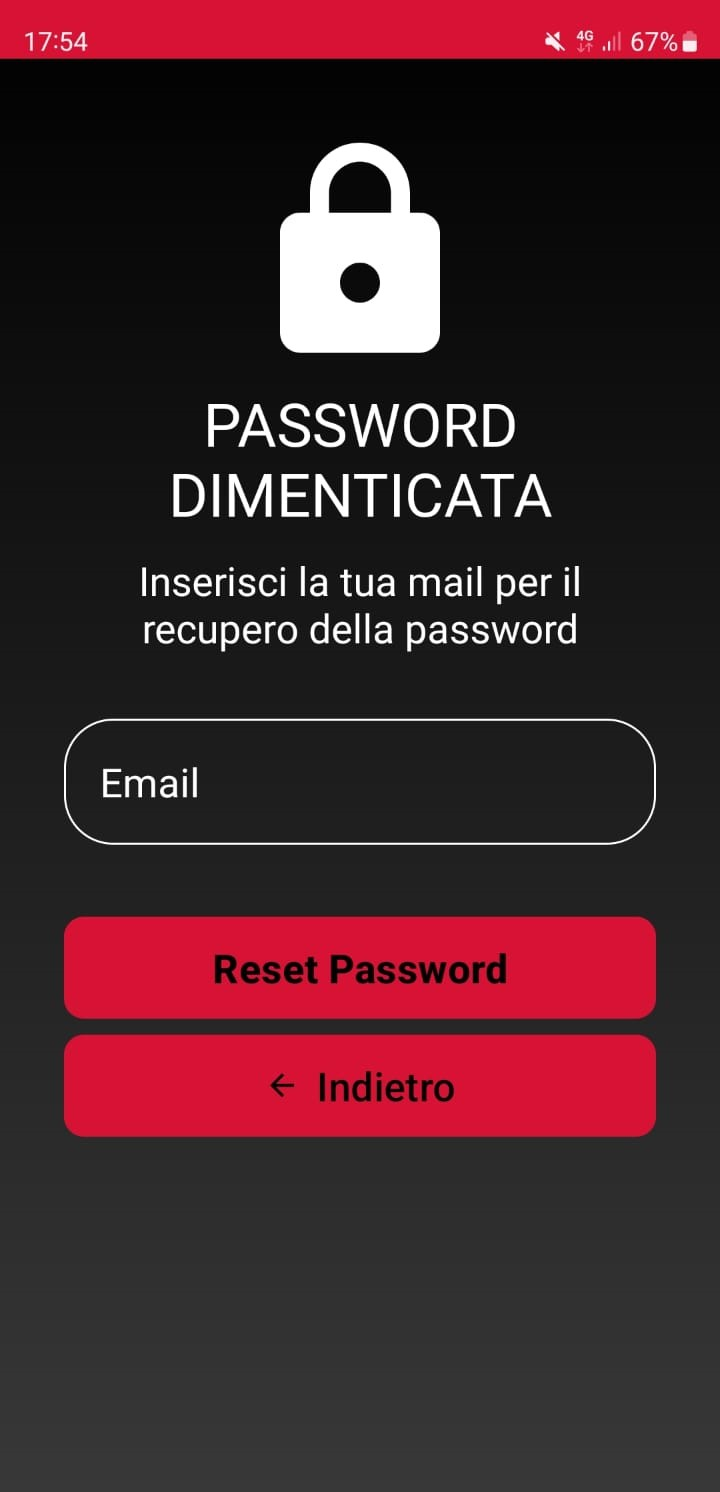
\includegraphics[width=\textwidth, height=0.45\textheight]{Immagini/App/pw_dimenticata_scuro.jpeg}
    \end{subfigure}
    \caption{Schermate di login con tema DARK.}
    \label{fig:dark1}
\end{figure}

\begin{figure}[ht]
    \centering
    \begin{subfigure}[b]{0.3\textwidth}
      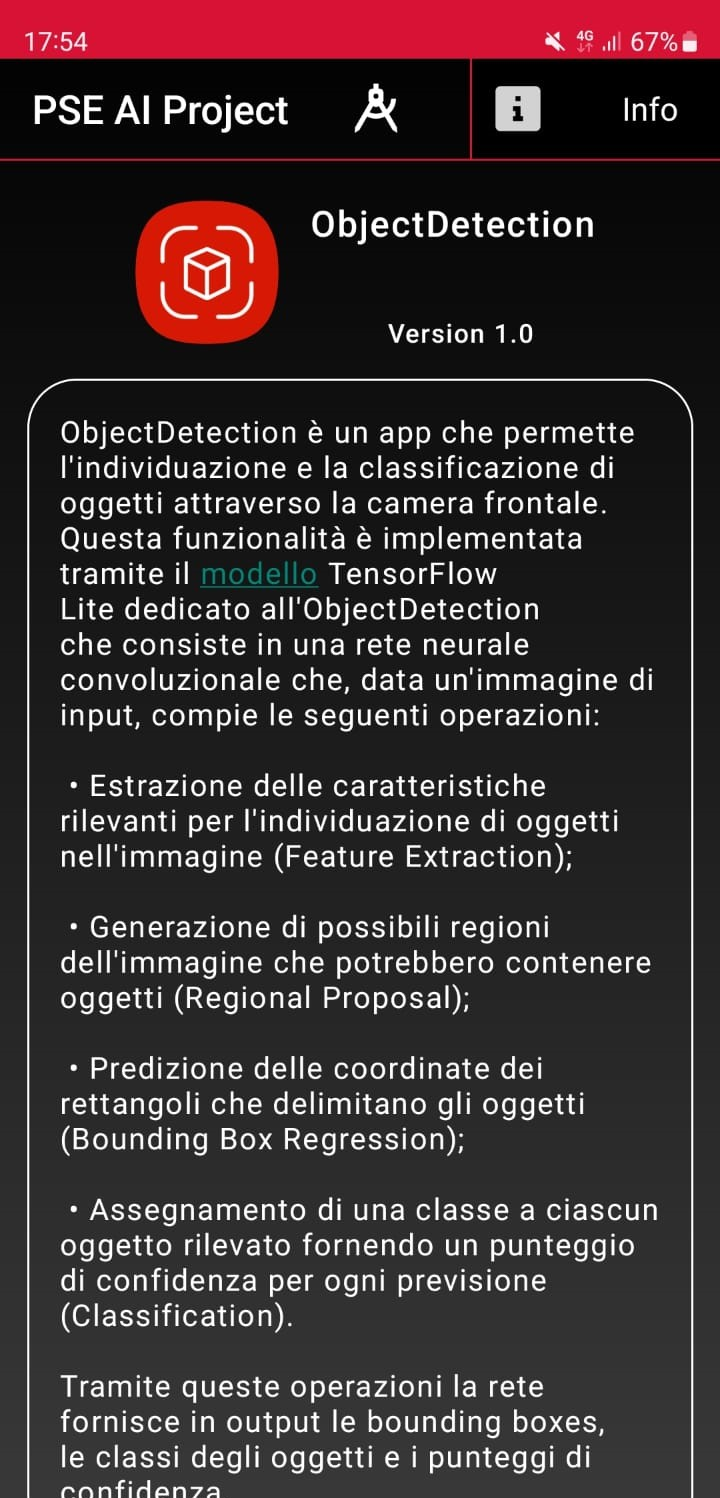
\includegraphics[width=\textwidth, height=0.45\textheight]{Immagini/App/info_scuro.jpeg}
    \end{subfigure}
    \begin{subfigure}[b]{0.3\textwidth}
      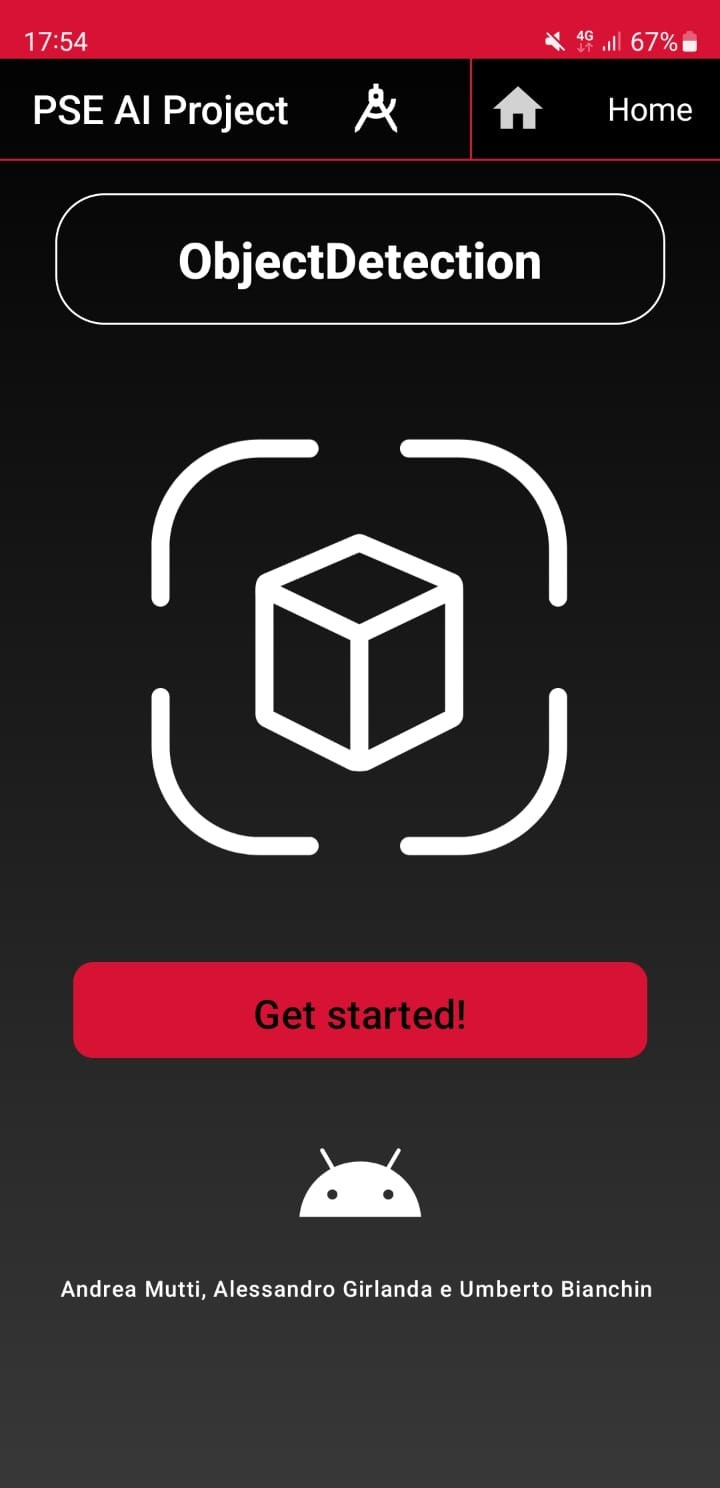
\includegraphics[width=\textwidth, height=0.45\textheight]{Immagini/App/home_scuro.jpeg}
    \end{subfigure}
    \caption{Schermate Info e Home con tema DARK.}
    \label{fig:dark2}
\end{figure}

\begin{figure}
    \centering
    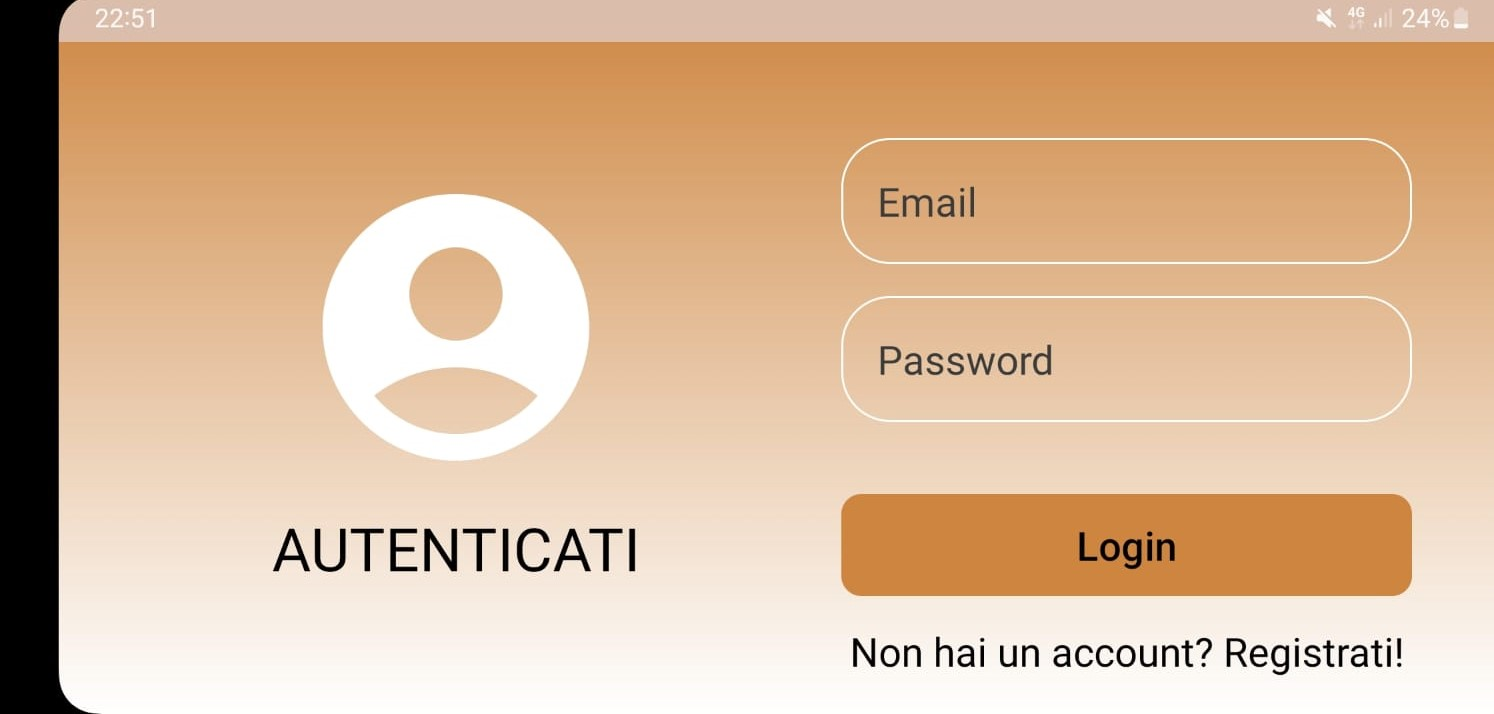
\includegraphics[width=0.5\textwidth]{Immagini/App/login_orizzontale.jpeg}
    \caption{Esempio di utilizzo del modello con 4 rettangoli.}
    \label{fig:orizzontale1}
\end{figure}

\begin{figure}
    \centering
    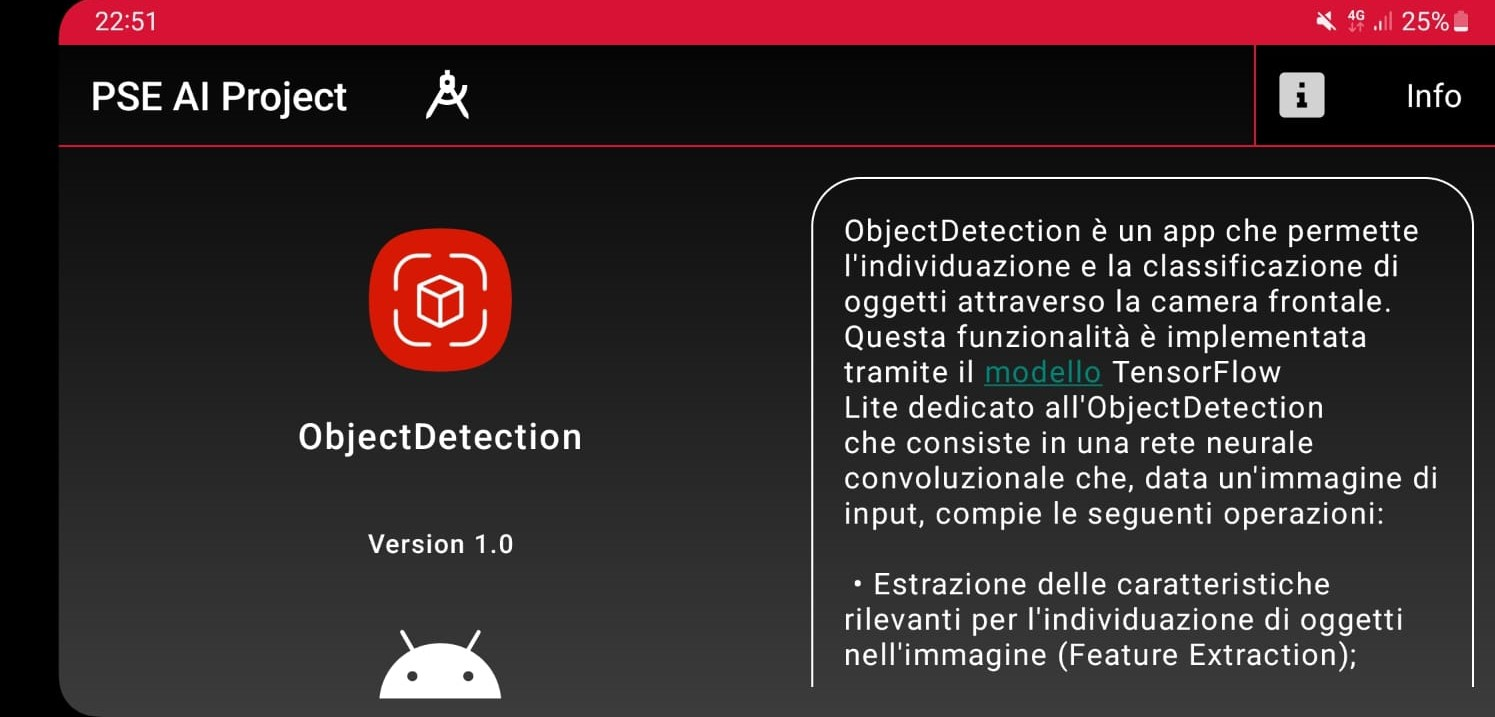
\includegraphics[width=0.5\textwidth]{Immagini/App/info_orizzontale.jpeg}
    \caption{Esempio di utilizzo del modello con 4 rettangoli.}
    \label{fig:orizzontale2}
\end{figure}

\begin{figure}[ht]
    \centering
    \begin{subfigure}[b]{0.3\textwidth}
      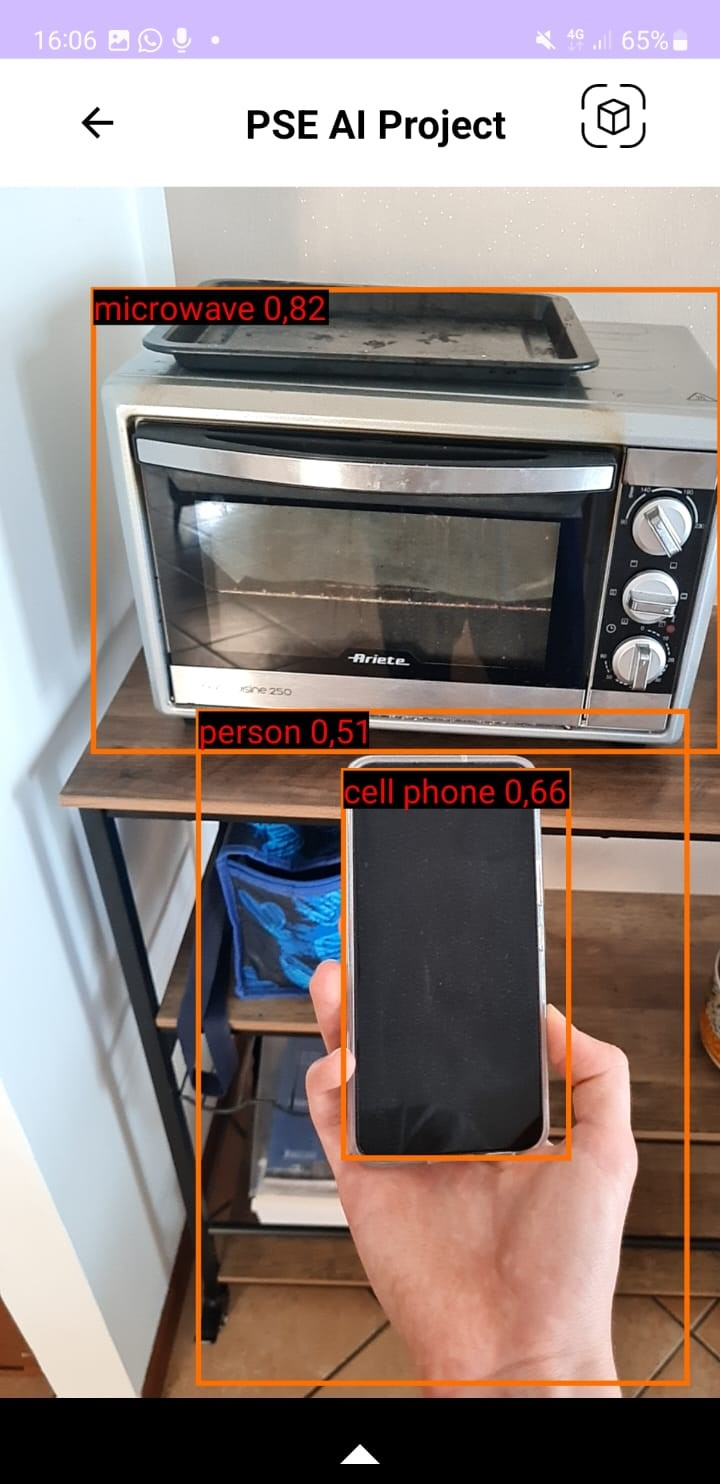
\includegraphics[width=\textwidth, height=0.45\textheight]{Immagini/App/funzionamento_3rettangoli.jpeg}
    \end{subfigure}
    \begin{subfigure}[b]{0.3\textwidth}
      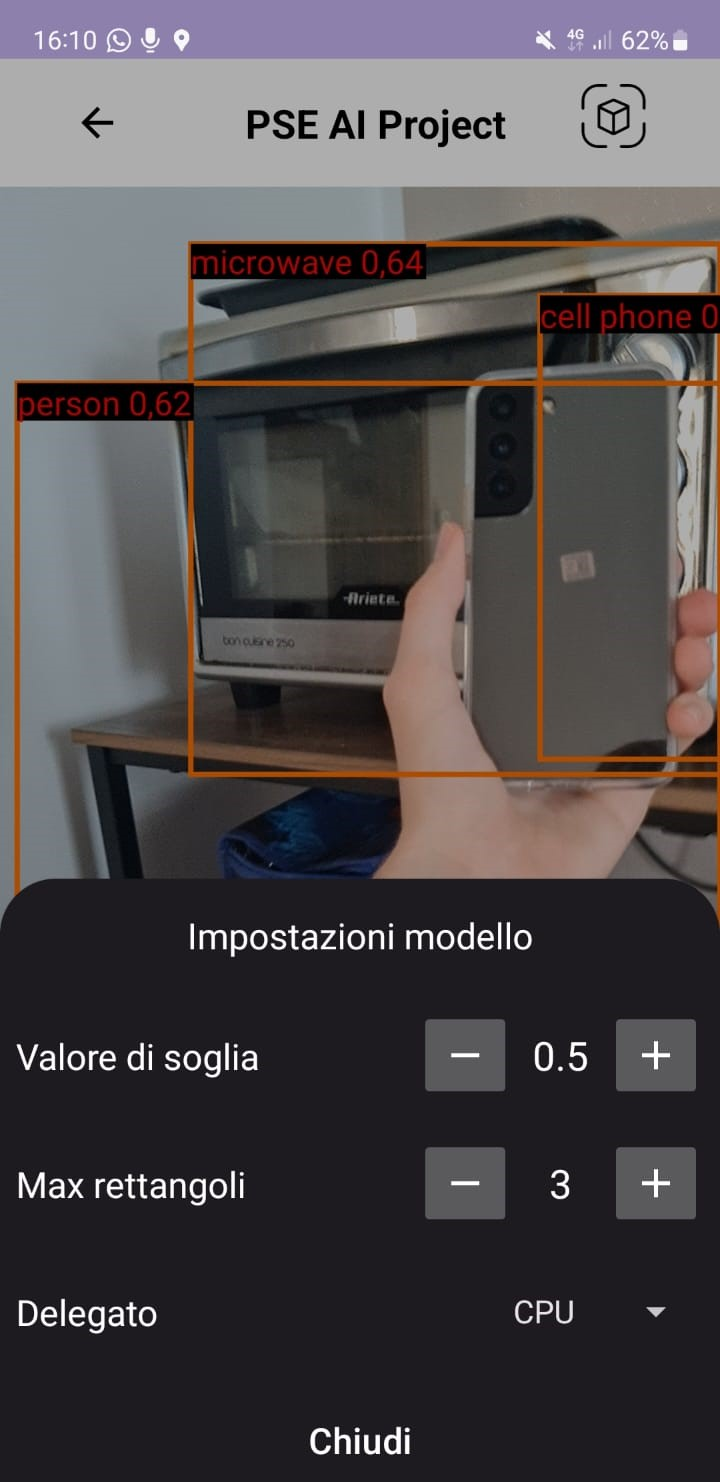
\includegraphics[width=\textwidth, height=0.45\textheight]{Immagini/App/funzionamento_impostazioni.jpeg}
    \end{subfigure}
    \caption{Esempio di utilizzo del modello e delle sue impostazioni.}
    \label{fig:funzionamento1}
\end{figure}

\begin{figure}
    \centering
    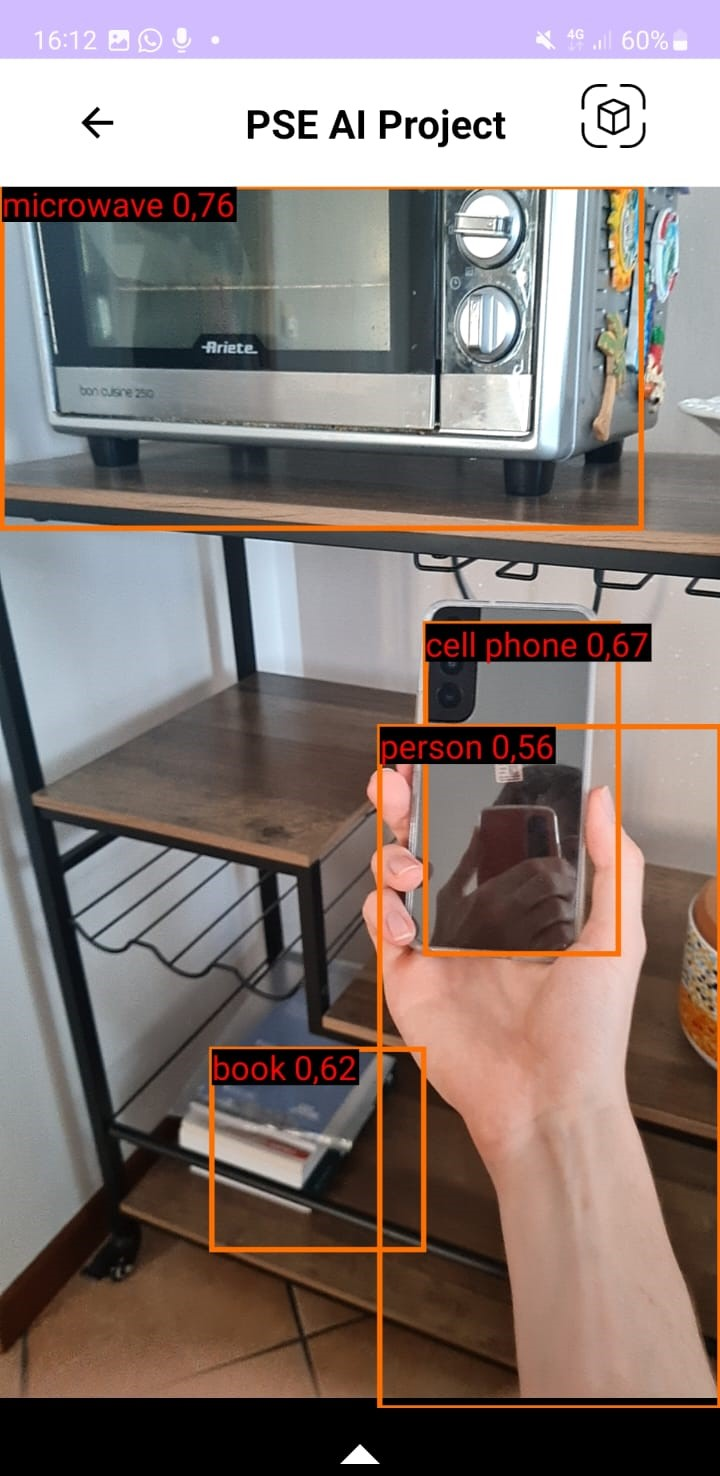
\includegraphics[width=0.3\textwidth]{Immagini/App/funzionamento_4rettangoli.jpeg}
    \caption{Esempio di utilizzo del modello con 4 rettangoli.}
    \label{fig:funzionamento2}
\end{figure}